\frame{
\large
\begin{enumerate}
\setcounter{enumi}{3}
 \item Resultados y Evaluación.
  \begin{itemize}
  \item Metodología.
  \item Expresividad y Cumplimiento de Criterios.
  \begin{enumerate}
   \item Punto de Vista Cuantitativo.
   \item Punto de Vista Cualitativo.
  \end{enumerate}
  \item Sistema MOLDEAS.
  \begin{enumerate}
   \item Consumo de Datos Enlazados Abiertos.
   \item Rendimiento de Consultas en SPARQL.
  \end{enumerate}
  \end{itemize}

\end{enumerate}

}


\frame{
  \frametitle{Metodología}

\begin{block}{Pasos de ejecución}
 \begin{enumerate}
\small
 \item Definición de los objetivos del experimento. 
\item Selección de una regla de asignación de las unidades experimentales a las condiciones de estudio. 
 \begin{itemize}
 \item Cualitativos: tipo de entorno hardware y software, etc.
   \item Cuantitativos: tamaño de la muestra, de la memoria y número de posibilidades de expresar una consulta.
\end{itemize}
 \item Especificación de las medidas de trabajo en cuanto a la respuesta.
 \item Especificación de un modelo.
 \item Ejecución de un experimento piloto. 
 \item Esquematización de los pasos a seguir. 
 \item Determinación del tamaño muestral.
 \item Revisión de las decisiones anteriores.
\end{enumerate}
\end{block}
}

\subsection*{Expresividad y Cumplimiento de Criterios}
\frame{
  \frametitle{Visión del experimento}

\begin{block}{Punto de Vista Cuantitativo}<1->
 ¿Cuál es la posibilidad de uso de datos enlazados para facilitar el \textbf{acceso} a un 
mayor número de recursos relacionados con los anuncios de licitación?
\end{block}

\begin{exampleblock}{Punto de Vista Cualitativo}<2->
Evaluación, grado de cumplimiento y comparación con otros enfoques de:
\begin{itemize}
 \item Principios de \opendata y \linkeddata.
 \item Buenas prácticas.
 \item Patrones de diseño.
 \item Características de pertenencia a la nube de datos enlazados y registro CKAN.
\end{itemize}
\end{exampleblock}
}

\frame{
\begin{block}{Expresividad}
Punto de Vista Cuantitativo.
\end{block}

}


\frame{
  \frametitle{Punto de Vista Cuantitativo}

\begin{block}{1-Definición de los objetivos del experimento}
\begin{enumerate}
 \item ¿Cuál es la expresividad actual, en términos de número de conceptos para realizar consultas, para el acceso a la información de anuncios de licitación?
 \item ¿Cuál es la ventaja de uso de un modelo RDF para la expresión y recuperación de la información de los anuncios de licitación?
 \item ¿Cómo favorecen los datos enlazados el aumento de expresividad en la ejecución de consultas y por tanto facilitan la recuperación de los 
anuncios de licitación? 
 \item ¿Cuál es el beneficio real del uso de datos enlazados para representar la información? 
 \item ¿Se incurre en algún error al aumentar la expresividad?
\end{enumerate}

\end{block}

}


\frame{
  \frametitle{Punto de Vista Cuantitativo}

\begin{block}{2-Selección de una regla de asignación de las unidades experimentales a las condiciones de estudio}<1->
\begin{enumerate}
\item Base documental $\mathcal{D}$ constituida por $1$ millón de anuncios de licitación.
\item Vocabulario controlado, $\mathcal{V}$, del CPV 2008, formado por $\#\mathcal{V} = 10357$ códigos/términos distintos.
\item Cada documento $d \in \mathcal{D}$, etiquetado con al menos un código $v \in \mathcal{V}$.
\item 9 Clasificaciones Estándar de Productos y Servicios.
\item Clasificación ``puente'': \textit{ProductOntology} (PO)
\end{enumerate}
\end{block}



}

\frame{
  \frametitle{Punto de Vista Cuantitativo}

\begin{block}{3-Especificación de las medidas de trabajo en cuanto a la respuesta}<1->
\begin{enumerate}
\item Nº de enlaces entre una PSC y el CPV 2008.
\item Nº de enlaces entre una PSC y el CPV 2008 a través de PO.
\item Ganancia de expresividad en términos porcentuales.
\end{enumerate}

\end{block}

\begin{exampleblock}{4-Especificación de un modelo}<2->
\begin{itemize}
\item El nuevo vocabulario controlado $\mathcal{V'}_{psc}$, enlazado con $\mathcal{V}_{psc}$, dispone de $\#\mathcal{V'}_{psc}$ términos.
\item La ganancia se calcula como: \begin{align}
\% =  \{ \langle (\#\mathcal{V'}_{psc}+\#\mathcal{V}) / \#\mathcal{V} \rangle - 1 \} * 100
\end{align}
\end{itemize}
\end{exampleblock}

}


\frame{
  \frametitle{Punto de Vista Cuantitativo}

\begin{block}{5-Ejecución de un experimento piloto}<1->
\begin{itemize}
 \item Sea $\mathcal{V} = \{ 1, 2, 3 \}$  y  $\mathcal{V}_{psc} = \{A, B, C, D, E\}$.
 \item El conjunto de pares enlaces es: $\{ (A,1), (B,2), (C,1) (E,2) \}$.
 \item Por tanto, el conjunto $\mathcal{V'}_{psc} = \{A, B, C, E\}$ y el \% de ganancia en expresividad será:
\begin{align}
\% =  \{ \langle (4+3) / 3 \rangle -1 \} * 100  =  133
\end{align}
\end{itemize}
\end{block}

\begin{exampleblock}{6-Esquematización de los pasos a seguir}<2->
\begin{enumerate}
\item Extracción de consultas en SPARQL para establecer el número de enlaces entre las mismas.
\item Procesamiento de los resultados mediante un \textit{script} para generar los resultados.
\end{enumerate}
\end{exampleblock}
}


\frame{
  \frametitle{Punto de Vista Cuantitativo}
\begin{alertblock}{Otros}
\begin{itemize}
 \item 7-Determinación del tamaño muestral (ya indicado en el punto 1).
 \item 8-Revisión de las decisiones anteriores.
\end{itemize}
\end{alertblock}
}



\frame{
    \frametitle{Punto de Vista Cuantitativo-Resultados Parciales}
\small
\begin{longtable}[c]{|l|l|l|l|l|p{1cm}|p{1cm}|} 
\hline
  $\mathcal{V}_{psc}$ & $\#\mathcal{V}_{psc}$  & $\#\mathcal{V'}_{psc}$ &$\#\mathcal{V'''}_{psc}$ &  $\%$ real &  $\%$ real \textit{PO}  &  $\%$ máx.   \\\hline
\endhead
CPV 2003 	& $8323$  	& $462$		& $8312$ 	& $4.46$ 	& $80.25$	& $80.36$  \\ \hline
CN 2012  	& $14552$	& $2390$	& $2390$ 	& $23.07$	& $23.07$	& $140.50$  \\ \hline
CPC 2008 	& $4408$	& $4402$   	& $4403$	& $42.50$	& $42.51$ 	& $42.56$  \\ \hline
CPA 2008 	& $5429$	& $5399$   	& $5410$	& $52.12$	& $52.23$	& $52.41$  \\ \hline
ISIC v4  	& $766$		& $765$   	& $765$ 	& $7.38$ 	& $7.38$	& $7.39$    \\ \hline
NAICS 2007 	& $2328$	& $2300$ 	& $2300$	& $22.20$	& $22.20$	& $22.47$  \\ \hline
NAICS 2012 	& $2212$	& $2186$ 	& $2186$	& $21.10$	& $21.10$	& $21.35$  \\ \hline
SITC v4 	& $4017$	& $3811$   	& $3820$	& $36.79$	& $36.88$	& $38.78$  \\ \hline
\multicolumn{7}{|c|}{\textbf{...}} \\ \hline
\hline
\end{longtable}
}

\frame{
  \frametitle{Punto de Vista Cuantitativo-Resultados Totales}
\small
\begin{longtable}[c]{|l|l|l|l|l|l|p{1cm}|} 
\hline
  \multicolumn{7}{|c|}{\textbf{Total}} \\ \hline
  $\mathcal{V}_{psc}$ & $\#\mathcal{V}_{psc}$  & $\#\mathcal{V'}_{psc}$ &$\#\mathcal{V'''}_{psc}$ &  $\%$ real &  $\%$ real \textit{PO}  &  $\%$ máx.   \\\hline
\endhead
$\star$ & $42035$ 		& $21715$   	& $29586$	& $209.66$ 	& $285.66$	& $405.86$ \\ \hline
\multicolumn{7}{|c|}{\textbf{Añadiendo enlaces entre CPV 2008 y \textit{Product Ontology-PO}}} \\ \hline
\textit{PO}& $\infty$	& $10000$   	& N/A	& $96.55$	& $96.55$ 	& $\infty$  \\ \hline
\multicolumn{7}{|c|}{\textbf{Total con vocabulario de \textit{Product Ontology}}} \\ \hline
$\star$	 & $\infty$	& $31715$   	& 39586	& $306.21$	& $382.21$	& $\infty$ \\ \hline
\hline
\end{longtable}

}


\frame{
  \frametitle{Punto de Vista Cuantitativo-Resultados}

\begin{figure}[!htb]
\centering
	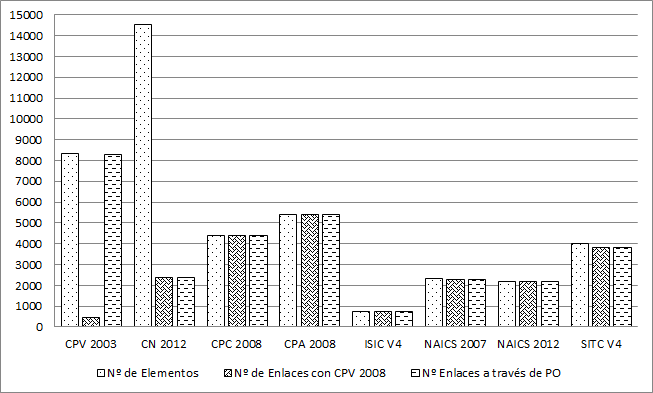
\includegraphics[width=10cm]{./imgs/pscs-enlaces}
\caption{Número de Elementos y Enlaces entre las PSCs y el CPV 2008.}
\end{figure}

}

\frame{
  \frametitle{Punto de Vista Cuantitativo-Resultados}

\begin{figure}[!htb]
\centering
	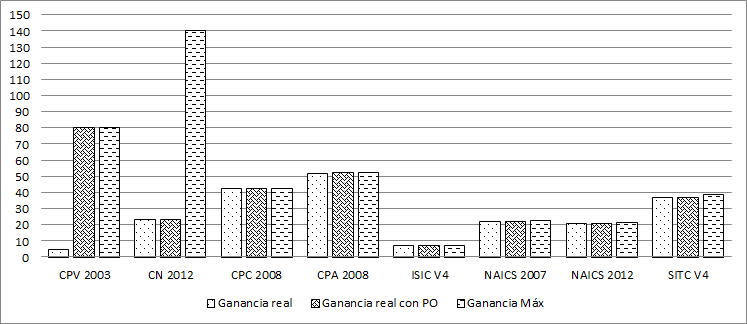
\includegraphics[width=10cm]{./imgs/pscs-ganancia}
\caption{Ganancia en expresividad.}
\end{figure}

}

\frame{
  \frametitle{Punto de Vista Cuantitativo-Resultados}

\begin{block}{Valoración}
 \begin{enumerate}
  \item Extensión del CPV 2008, $10357$ términos, hasta:
 \begin{itemize}
  \item $21715$ términos, con enlaces entre las PSCs y el CPV 2008.
  \item $29586$ términos, con enlaces entre las PSCs y el CPV 2008 a través de \textit{PO}.
 \end{itemize}
  \item Se establece un:
   \begin{itemize}
    \item \textbf{$8.65\%$} y \textbf{$6.64\%$} (PO) de enlaces exactos.
    \item \textbf{$91.35\%$} y \textbf{$93.36\%$} (PO) de enlaces automáticos.
   \end{itemize}
 \item Cifras de ganancia:
  \begin{itemize}
  \item Real: $209.66\%$.
  \item Real con \textit{PO}: $285.66\%$
  \item Máximo: $405.86\%$.
 \end{itemize}
  \item Los enlaces y la reconciliación de entidades se realizan bajo un umbral $\mu$ ($n$ primeros resultados normalizados).
 \end{enumerate}
\end{block}


}

\frame{
  \frametitle{Punto de Vista Cuantitativo-Resultados}

\begin{figure}[!htb]
\centering
	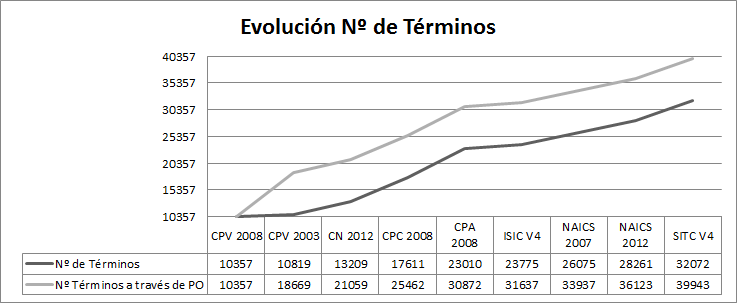
\includegraphics[width=11cm]{./imgs/evo-n-terminos}
\caption{Evolución Número de Términos.}
\label{fig:eval-n-terminos}
\end{figure}

}


\frame{
  \frametitle{Punto de Vista Cuantitativo-Conclusiones}

\begin{exampleblock}{Puntos Clave}
\begin{itemize}
 \item \textbf{Aumento} del \textbf{vocabulario de entrada} del CPV 2008 con \linkeddata.
 \item \textbf{Mejora} de la \textbf{expresividad} para la realización de consultas en SPARQL.
 \item \textbf{Incremento} del número de \textbf{anuncios} de licitación a los que se puede \textbf{acceder}.
 \item \textbf{Establecimiento} de una \textbf{fórmula} para el cálculo de la \textbf{ganancia} del enlazado de datos.
\end{itemize}
\end{exampleblock}
}

%%%%%%%%%
%%%%%%%%	punto de vista cualitativo
%%%%%%%%


\frame{
\begin{exampleblock}{Cumplimiento de Criterios}
Punto de Vista Cualitativo. 
\end{exampleblock}
}



\frame{
  \frametitle{Punto de Vista Cualitativo}

\begin{block}{1-Definición de los objetivos del experimento}
\begin{enumerate}
 \item ¿El ciclo de vida seguido y los datos generados certifican la aplicación de buenas prácticas y principios de \linkeddata?
 \item ¿Qué nivel del modelo de 5 $\star$ se puede establecer?
 \item ¿Qué porcentaje de patrones de diseño se han aplicado en los datos generados?
 \item ¿Los datos generados pueden pertenecer a la nube de datos enlazados abiertos?
 \item ¿Los datos generados pueden pertenecer a un registro CKAN? 
 \item ¿Se certifica el cumplimiento de los principios de \opendata?
 \item ¿Se puede asegurar que los datos son enlazados y abiertos?
 \item ¿Qué beneficios se obtienen del cumplimiento de estos objetivos?
\end{enumerate}

\end{block}

}

\frame{
  \frametitle{Punto de Vista Cualitativo}

\begin{block}{2-Selección de una regla de asignación de las unidades experimentales a las condiciones de estudio}<1->
\begin{enumerate}
\item \textit{Dataset} RDF de los anuncios de licitación pública.
\begin{itemize}
 \item Boletines y Publicaciones oficiales: TED y BOE.
 \item Plataformas de contratación: AGE.
 \item Servicios de terceros: Euroalert.net y Licitaciones.es
 \item Basados en semántica: LOTED.
\end{itemize}
\item \textit{Dataset} RDF de las PSCs.
\begin{itemize}
 \item Publicaciones oficiales: UE, ONU, etc.
 \item Servicios de terceros.
\end{itemize}
\item \textit{Dataset} RDF de las organizaciones.
\begin{itemize}
 \item Boletines y Publicaciones oficiales: TED y BORME.
 \item Plataformas de contratación: AGE.
 \item Servicios y BBDD de terceros.
 \item Basadas en \opendata: OpenCorporates.
\end{itemize}
\end{enumerate}
\end{block}


}


\frame{
  \frametitle{Punto de Vista Cualitativo}

\begin{block}{3-Especificación de las medidas de trabajo en cuanto a la respuesta}
\begin{enumerate}
 \item Valor positivo, \si, si es un criterio que debe tener y se cumple (\textbf{173}).
 \item Valor negativo, \no, si es un criterio que debe tener y no se cumple (\textbf{0}).
 \item Valor no aplicable, \na, si es un criterio que se desconoce, que se solapa con otro o no está asociado a ese enfoque (\textbf{23}).
\end{enumerate}
\end{block}

}


\frame{
  \frametitle{Punto de Vista Cualitativo}
\begin{exampleblock}{Diseño de Tablas de Validación}
\begin{itemize}
\item $T^{1}$-Tabla de Validación de Características \linkeddata.
\item $T^{2}$-\ldots de \textit{Linked Data Patterns}.
\item $T^{3}$-\ldots de Principios de \linkeddata.
\item $T^{3}_1$-\ldots del Modelo $\star$.
\item $T^{4}$-\ldots de Principios de \opendata.
\item $T^{4}_1$-\ldots sobre Características de \opendata.
\item $T^{5}$-\ldots sobre Características para pertenecer a la nube de \lod.
\item $T^{6}$-\ldots para registrar el \dataset en CKAN.
\end{itemize}
\end{exampleblock}

}

\frame{
  \frametitle{Punto de Vista Cualitativo}

\begin{block}{4-Especificación de un modelo}<1->
No aplicable.
\end{block}

\begin{exampleblock}{5-Ejecución de un experimento piloto}<2->
Valoración inicial con sólo un conjunto de datos.
\end{exampleblock}

\begin{alertblock}{6-Esquematización de los pasos a seguir}<3->
\begin{enumerate}
 \item Establecimiento del modelo de referencia, con los valores admitidos.
 \item Revisión uno a uno de los criterios.
 \item Agregación de los resultados y valoraciones.
 \item Extracción de estadísticas, contraste de hipótesis, validación y evaluación.
\end{enumerate}
\end{alertblock}
}


\frame{
  \frametitle{Punto de Vista Cualitativo}
\begin{block}{Otros}
\begin{itemize}
 \item 7-Determinación del tamaño muestral (ya indicado en el punto 1).
 \item 8-Revisión de las decisiones anteriores.
\end{itemize}
\end{block}
}





\frame{
  \frametitle{Punto de Vista Cualitativo-Resultados en \%}
\small
\begin{longtable}[c]{|p{2.25cm}|c|c|c|c|c|c|c|c|}
\hline
\textbf{Versión}&$T^{1}$ & $T^{2}$& $T^{3}$ & $T^{3}_1$ & $T^{4}$ & $T^{4}_1$ &$T^{5}$ & $T^{6}$ \\ \hline
\endhead
 \multicolumn{9}{|c|}{\textbf{Anuncios de Licitación}} \\ \hline
 \textbf{TED}	     			& $65$ & \na & $100$ & $100$ & $75$ & $78,57$ & \na & \na \\ \hline
 \textbf{Plataforma de Contratación}	& $75$ & \na & $100$ & $100$ & $87,5$ & $78,57$ & \na & \na \\ \hline 
 \textbf{BOE}	     			& $52,63$ & \na & $100$ & $100$ & $100$ & $76,92$ & \na & \na\\ \hline 
 \textbf{Servicios Externos}	     	& $60$ & \na & $100$ & $100$ & $62,5$ & $66,66$ & \na & \na \\ \hline 
 \textbf{LOTED}	     			& $59,32$ & $74,19$ & $100$ & $100$ & $100$ & $85,71$ & $100$ & \na \\ \hline 
 \textbf{MOLDEAS}	     		& $88,52$ & $91,18$ & $100$ & $100$ & $100$ & $100$ & $100$ & \na \\ \hline 
\hline
\end{longtable} 

}

\frame{
  \frametitle{Punto de Vista Cualitativo-Resultados en \%}
\small
 \begin{longtable}[c]{|p{2cm}|c|c|c|c|c|c|c|c|}
\hline
\textbf{Versión}&$T^{1}$ & $T^{2}$& $T^{3}$ & $T^{3}_1$ & $T^{4}$ & $T^{4}_1$ &$T^{5}$ & $T^{6}$ \\ \hline
\endhead
 \multicolumn{9}{|c|}{\textbf{Catálogo de Clasificaciones de Productos}} \\ \hline
 \textbf{CSV/ MSExcel} 			&$69,23$ & \na & \na & $100$ & $100$ & $42,86$ & \na & \na \\ \hline 
 \textbf{Servicios on-line}  		&$50$ & \na & \na & \na & $71,43$ & $38,46$ & \na & \na \\ \hline 
 \textbf{MOLDEAS}			&$88,52$ & $100$ & $100$ & $100$ & $100$ & $100$ & $100$ & $100$ \\ \hline 
\hline
\end{longtable} 


}
\frame{
  \frametitle{Punto de Vista Cualitativo-Resultados en \%}
\small
\begin{longtable}[l]{|p{2.25cm}|c|c|c|c|c|c|c|c|}
\hline
\textbf{Versión}&$T^{1}$ & $T^{2}$& $T^{3}$ & $T^{3}_1$ & $T^{4}$ & $T^{4}_1$ &$T^{5}$ & $T^{6}$ \\ \hline
\endhead
 \multicolumn{9}{|c|}{\textbf{Organizaciones}} \\ \hline
 \textbf{TED} 				& $50$ & \na & \na & $100$ & $75$ & $71,43$ & \na & \na \\ \hline 
 \textbf{Plataforma de Contratación} 	& $76,47$ & \na & $100$ & $20$ & $100$ & $85,71$ & \na & \na\\ \hline 
 \textbf{BORME}			 	& $100$ & \na & \na & $100$ & $100$ & $92,85$ & \na & \na \\ \hline 
 \textbf{Servicios Externos} 		& $60$ & \na & $100$ & $100$ & $12,5$ & $50$ & \na & \na \\ \hline 
 \textbf{BBDD externa} 			& $100$ & \na & \na & \na & $16,67$ & $71,43$ & \na & \na \\ \hline 
 \textbf{Open Corporates} 	 	& $61,40$ & $67,74$ & $100$ & $100$ & $100$ & $92,86$ & $100$ & \na\\ \hline 
 \textbf{MOLDEAS} 		 	& $88,52$ & $91,18$ & $100$ & $100$ & $100$ & $100$ & $100$ & \na \\ \hline 
\hline
\end{longtable} 

}

\frame{
  \frametitle{Punto de Vista Cualitativo-Resultados}

\begin{figure}[!htb]
\centering
	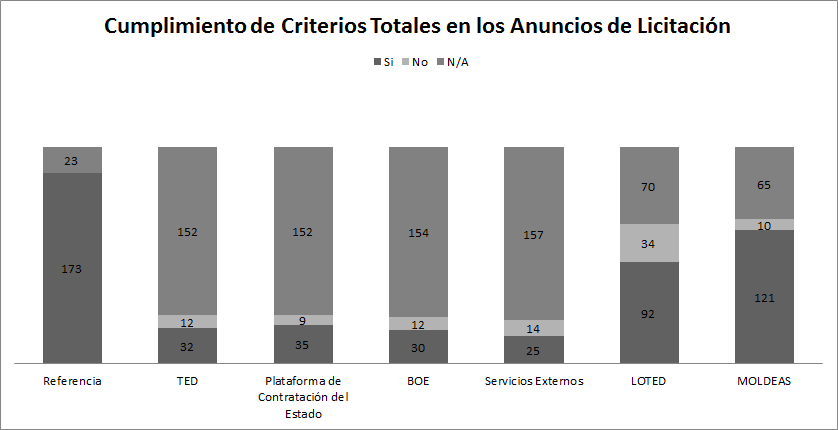
\includegraphics[width=11cm]{./imgs/criterios-total-ppn}
\end{figure}

}

\frame{
  \frametitle{Punto de Vista Cualitativo-Resultados}

\begin{figure}[!htb]
\centering
	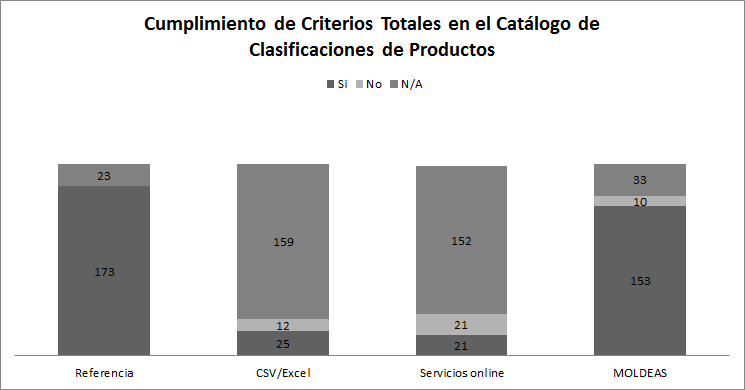
\includegraphics[width=11cm]{./imgs/criterios-total-pscs}
\end{figure}

}
\frame{
  \frametitle{Punto de Vista Cualitativo-Resultados}
\begin{figure}[!htb]
\centering
	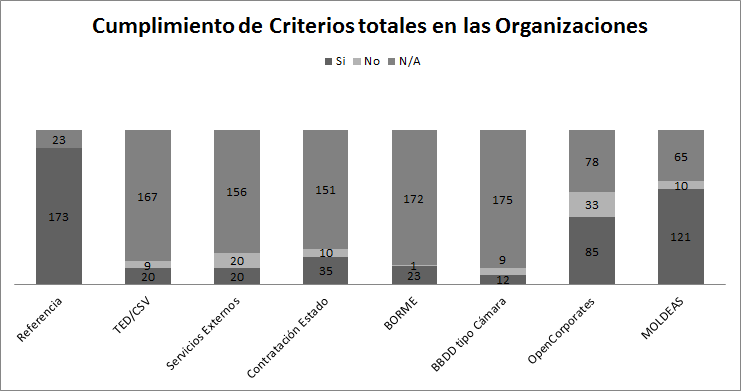
\includegraphics[width=11cm]{./imgs/criterios-total-orgs}
\end{figure}

}



\frame{
  \frametitle{Punto de Vista Cualitativo-\linebreak Resultados en \% \si entre aplicables}
\small
\begin{longtable}[c]{|p{2.25cm}|c|c|c||c||c|} 
\hline
 \textbf{Versión} & \si&\no&\na & \textbf{Total} & \textbf{\% \si entre aplicables} \\\hline
\endhead
    \textbf{Referencia} & 173 & 0 & 23 & 196& 100 \\ \hline \hline
 \multicolumn{6}{|c|}{\textbf{Anuncios de Licitación}} \\ \hline   
     \textbf{TED} & 32 & 12 & 152 &`` & $72.72$\\ \hline 
     \textbf{Plataforma de Contratación} & 35 & 9 & 152 &`` & $79.54$\\ \hline 
    \textbf{BOE} & 30 & 12 & 154 &`` & $71.42$\\ \hline 
    \textbf{Servicios Externos} & 25 & 14 & 157 &`` & $64.10$\\ \hline 
    \textbf{LOTED} & 92 & 34 & 70 &`` & $73.01$\\ \hline 
     \textbf{MOLDEAS} & 121 & 10 & 65 &`` & $92.36$\\ \hline 
\hline
\end{longtable}
}


\frame{
  \frametitle{Punto de Vista Cualitativo-\linebreak Resultados en \% \si entre aplicables}
\small
\begin{longtable}[c]{|p{2cm}|c|c|c||c||c|} 
\hline
 \textbf{Versión} & \si&\no&\na & \textbf{Total} & \textbf{\% \si entre aplicables} \\\hline
\endhead
    \textbf{Referencia} & 173 & 0 & 23 & 196& 100 \\ \hline \hline
 \multicolumn{6}{|c|}{\textbf{Catálogo de Clasificaciones de Productos}} \\ \hline
    \textbf{CSV/ MSExcel} &  25 & 12 & 159 &`` & $67.56$\\ \hline 
     \textbf{Servicios on-line} &  21 & 21 & 154 &`` & $50$\\ \hline 
    \textbf{MOLDEAS} &  166 & 7 & 23 &`` & $93.86$\\ \hline 

\hline
\end{longtable}
}


\frame{
  \frametitle{Punto de Vista Cualitativo-\linebreak Resultados en \% \si entre aplicables}
\small
\begin{longtable}[c]{|p{2.25cm}|c|c|c||c||c|} 
\hline
 \textbf{Versión} & \si&\no&\na & \textbf{Total} & \textbf{\% \si entre aplicables} \\\hline
\endhead
    \textbf{Referencia} & 173 & 0 & 23 & 196& 100 \\ \hline \hline
 \multicolumn{6}{|c|}{\textbf{Organizaciones}} \\ \hline
    \textbf{TED} & 20 & 9 & 167 &`` & $68.96$\\ \hline 
    \textbf{Plataforma de Contratación}  & 35 & 10 & 151 &`` & $77.77$ \\ \hline 
    \textbf{BORME}  & 23 & 1 & 172 &``& $95.83$\\ \hline 
    \textbf{Servicios Externos}  & 20 & 20 & 156 &`` & $50$\\ \hline   
    \textbf{BBDD externa}  & 12 & 9 & 175 &`` & $57.14$\\ \hline 
    \textbf{Open Corporates}  & 85 & 33 & 78  &`` & $72.03$\\ \hline 
    \textbf{MOLDEAS}  & 121 & 10 & 65 &`` & $92.36$\\ \hline 
\hline
\end{longtable}
}









\frame{
  \frametitle{Punto de Vista Cualitativo-Resultados}

\begin{block}{Valoración}
 \begin{enumerate}
\item El ciclo de vida asegura los principios y criterios de \linkeddata y \opendata.
\item Se establece un nivel de $5\star$ para los \datasets transformados.
\item Se ha aplicado un alto porcentaje de patrones de diseño, calidad implícita para la reutilización de datos.
\item Los \datasets transformados pueden pertenecer a la nube de \lod y a un registro CKAN.
\item En general, el enfoque de MOLDEAS mejora cualitativamente la información y datos respecto a otros enfoques.
 \end{enumerate}
\end{block}
}


\frame{
  \frametitle{Punto de Vista Cualitativo-Conclusiones}
\begin{exampleblock}{Puntos Clave}
\begin{itemize}
\small
 \item \textbf{Mejora} \textbf{cualitativa} la información y datos.
 \item \textbf{Aumento} de la visión global de los datos, \textbf{expresividad} y \textbf{estructuración}.
 \item \textbf{Aplicación} intensiva de \textbf{estándares}.
 \item \textbf{Incremento} del \textbf{conocimiento} en el dominio de \eproc.
 \item \textbf{Impulso} de la \textbf{reutilización} de la \textbf{información} y datos, mayor poder de redistribución.
 \item \textbf{Minimización} de \textbf{restricciones} tecnológicas.
 \item \textbf{Minimización} de \textbf{aspectos discriminatorios}.
 \item \textbf{Aumento} de la \textbf{transparencia}, \textbf{inclusión} y \textbf{responsabilidad}.
 \item \textbf{Alineación} con las actuales \textbf{propuestas estratégicas} de futuro.
 \item \ldots
\end{itemize}
\end{exampleblock}
}

\subsection*{Sistema MOLDEAS}
\frame{
\begin{exampleblock}{Sistema MOLDEAS}
Consumo de Datos Enlazados Abiertos. 
\end{exampleblock}
}


\frame{
  \frametitle{Consumo de Datos Enlazados Abiertos}

\begin{exampleblock}{Objetivos Generales}<1->
 \begin{itemize}
\small
 \item Consumir los datos enlazados desde un lenguaje de programación.
 \item Crear un sistema de recuperación de información.
\end{itemize}
\end{exampleblock}


\begin{block}{1-Definición de los objetivos del experimento}<2->
\begin{enumerate}
\small
 \item ¿Es posible implementar un sistema de recuperación de información utilizando datos enlazados?
 \item ¿Es posible explotar las relaciones semánticas establecidas para mejorar la recuperación de información?
 \item ¿Cuál es el mejor enfoque para la recuperación de información en los anuncios de licitación? 
 \item ¿Cómo afectan los resultados en la implementación actual del sistema MOLDEAS?
\end{enumerate}

\end{block}

}


\frame{
  \frametitle{Consumo de Datos Enlazados Abiertos}

\begin{block}{2-Selección de una regla de asignación de las unidades experimentales a las condiciones de estudio}
\begin{enumerate}
 \item Unidad experimental de este estudio será un repositorio RDF.
\item Base documental $\mathcal{D}$ constituida por $1$ millón de anuncios de licitación.
\item Vocabulario controlado, $\mathcal{V}$, del CPV 2008, formado por 10357 códigos/términos distintos.
\item Cada documento $d \in \mathcal{D}$, etiquetado con al menos un código $v \in \mathcal{V}$.
\item $11$ consultas, $Q_{str}$, proporcionadas por Euroalert.net.
\item Las medidas de evaluación dependen del nº de códigos CPV generados por MOLDEAS.
\end{enumerate}
\end{block}

}

\frame{
  \frametitle{Consumo de Datos Enlazados Abiertos}
\small
\begin{longtable}[c]{|l|p{6cm}|p{3cm}|} 
\hline
\textbf{$Q_{i}$} &  \textbf{Consulta de Usuario-$Q_{str}$} &  \textbf{Nº de Códigos CPV relevantes-$\#Q^{i}_{cpv}$} \\\hline
\endhead
$Q_1$ & \ldots & $463$ \\ \hline
$Q_2$ & \ldots & $35$ \\ \hline
$Q_3$ & \ldots & $7$ \\ \hline
$Q_4$ & \ldots & $26$ \\ \hline
$Q_5$ & \ldots &  $277$\\ \hline
\multicolumn{3}{|c|}{\textbf{...}} \\ \hline
 \hline
\end{longtable}

}

\frame{
  \frametitle{Consumo de Datos Enlazados Abiertos}
\small
\begin{longtable}[c]{|l|p{6cm}|p{3cm}|} 
\hline
\textbf{$Q_{i}$} &  \textbf{Consulta de Usuario-$Q_{str}$} &  \textbf{Nº de Códigos CPV relevantes-$\#Q^{i}_{cpv}$} \\\hline
\endhead
$Q_6$ & \ldots & $1$ \\ \hline
$Q_7$ & \ldots & $117$ \\ \hline
$Q_8$ & \ldots & $13$ \\ \hline
$Q_9$ & \ldots & $10$ \\ \hline
$Q_{10}$ & \ldots &  $173$\\ \hline
$Q_{11}$ & \ldots &  $13$\\ \hline
 \hline
\end{longtable}

}

\frame{
  \frametitle{Consumo de Datos Enlazados Abiertos}
\small
\begin{longtable}[c]{|l|p{5cm}|p{3.5cm}|} 
\hline
\textbf{Método} &  \textbf{Descripción} &  \textbf{Tecnología} \\\hline
\endhead
$M^1$ & Se indexan las descripciones de los códigos CPV y proceso de búsqueda sintáctica de las consultas $Q_{i}$. & Apache Lucene y Solr \\ \hline
$M^2$ & Se extraen una serie de códigos CPV candidatos según jerarquía. & $M^1$ + ponderación \textit{broader/ narrower} \\ \hline
$M^3$ & \ldots según jerarquía con \textit{Spreading Activation}. & $M^1$ + ONTOSPREAD \\ \hline
$M^4$ & \ldots según histórico de las relaciones entre códigos de los anuncios previos. & $M^1$ + Apache Mahout \\ \hline
\hline
\end{longtable}

}

 
 
 \frame{
\frametitle{Consumo de Datos Enlazados Abiertos}
 
 \begin{block}{3-Especificación de las medidas de trabajo en cuanto a la respuesta}<1->
\begin{enumerate}
\item Para cada consulta se recogen los códigos CPV 2008 generados.
\item Se comparan con los indicados en las consultas $Q_{i}$.
\item Se obtienen las medidas Precisión, \textit{Recall}, \textit{Accuracy} y \textit{Specificity} (\textit{PRAS}).
\end{enumerate}

\end{block}

\begin{exampleblock}{5-Ejecución de un experimento piloto}<2->
En primer lugar se realiza una consulta para verificar el proceso de búsqueda en cada método 
y la obtención de medidas.
\end{exampleblock}

}

 \frame{
\frametitle{Consumo de Datos Enlazados Abiertos}
 
 \begin{block}{6-Esquematización de los pasos a seguir}<1->
\begin{enumerate}
 \item A cada consulta $Q_{str}$, identificada como $Q_{i}$, se le aplica un método $M^{i}$, devuelve al $\#Q^{i}_{cpv}$ elementos.
 \item Cada conjunto resultado $Q^{M^i}_{cpv}$ se compara con el conjunto esperado $Q^{i}_{cpv}$ con un \textit{script}.
 \item Se generan los valores \textit{PRAS} para cada método $M^{i}$ y consulta de entrada $Q_{i}$.
\end{enumerate}

\end{block}

 \begin{alertblock}{Otros}<2->
\begin{enumerate}
  \item 4-Especificación de un modelo (N/A).
  \item 7-Determinación del tamaño muestral (ya indicado en el punto 1).
  \item 8-Revisión de las decisiones anteriores.
\end{enumerate}

\end{alertblock}

}

 \frame{
   \frametitle{Consumo de Datos Enlazados Abiertos-\linebreak Resultados Agregados ($\bar{X}$)}
 
\small
\begin{longtable}[c]{|l|c|c|c|c|} 
\hline
\textbf{Método} &  \textbf{Precisión} & \textbf{Recall} & \textbf{Accuracy} & \textbf{Specificity} \\\hline
\endhead
$M^1$ &  $0,28$ & $0,26$ & $0,99$ & $1,00$ \\ \hline
$M^2$ &  $0,11$ & $0,11$ & $0,98$ & $0,99$   \\ \hline
$M^3$ &  $0,23$ & $0,23$ & $0,99$ & $1,00$  \\ \hline
$M^4$ &  $0,03$ & $0,03$ & $0,96$ & $0,98$\\ \hline
\hline
\end{longtable}

}

\frame{
  \frametitle{Consumo de Datos Enlazados Abiertos-Resultados}

\begin{block}{Valoración}
 \begin{enumerate}
\item El tipo y formato de una fuente de datos no es impedimento para la construcción de servicios 
en un dominio determinado.
\item Las relaciones semánticas de los datos se pueden explotar para recuperar información.
\item El enfoque tradicional sintáctico, $M^1$, se comporta más cercano a las expectativas del usuario.
 \end{enumerate}
\end{block}
}
% 

\frame{
  \frametitle{Consumo de Datos Enlazados Abiertos-Conclusiones}

\begin{exampleblock}{Principal Punto Clave}
La \textbf{casuística} de un sistema de soporte a la decisión o de recuperación a la información 
en \textbf{\eproc} es muy \textbf{compleja}, existen \textbf{muchas} \textbf{variables} de \textbf{información} que se pueden optimizar.
\end{exampleblock}
}


\frame{
\begin{exampleblock}{Sistema MOLDEAS}
Rendimiento de Consultas en SPARQL.
\end{exampleblock}
}


\frame{
  \frametitle{Rendimiento de Consultas en SPARQL}

\begin{exampleblock}{Objetivo General}<1->
Mejorar el rendimiento de las consultas en SPARQL.
\end{exampleblock}


\begin{block}{1-Definición de los objetivos del experimento}<2->
\begin{enumerate}
 \item ¿Cuáles son las mejoras que se pueden aplicar sobre una consulta en SPARQL para mejorar el tiempo de ejecución?
 \item ¿Cuál es la combinación de mejoras que obtiene un mejor tiempo de respuesta?
 \item ¿Cuál es el coste de la combinación de estas mejoras? 
 \item ¿Existe algún elemento externo de configuración que implique un incremento en el tiempo de ejecución de las consultas? 
 \item ¿Cómo afectan los resultados en la implementación actual del sistema MOLDEAS?
\end{enumerate}

\end{block}

}
% 

\frame{
  \frametitle{Rendimiento de Consultas en SPARQL}

\begin{block}{2-Selección de una regla de asignación de las unidades experimentales a las condiciones de estudio}
\begin{enumerate}
\item Unidad experimental de este estudio será un repositorio RDF.
\item Base documental $\mathcal{D}$ constituida por $1$ millón de anuncios de licitación.
\item Vocabulario controlado, $\mathcal{V}$, del CPV 2008, formado por 10357 códigos/términos distintos.
\item Cada documento $d \in \mathcal{D}$, etiquetado con al menos un código $v \in \mathcal{V}$ y un códigos NUTS.
\item Casos de test $T_k$ (tratamiento) para cada consulta $Q_k$ con características $F_k$.
\item Ejecución de 3 réplicas por cada $T_k$ con reinicio y calentamiento del entorno de pruebas.
\end{enumerate}
\end{block}

}


 \frame{
  \frametitle{Rendimiento de Consultas en SPARQL}
 
 \begin{block}{3-Especificación de las medidas de trabajo en cuanto a la respuesta}<1->
 Tiempo de ejecución en segundos.
\end{block}

\begin{exampleblock}{5-Ejecución de un experimento piloto}<2->
\begin{itemize}
 \item Una muestra de consultas, sólo un año de anuncios de licitación. 
  \item Ejecución de todos los tratamientos.
 \item Toma de tiempos y obtención de resultados.
\end{itemize}
\end{exampleblock}

}

 \frame{
  \frametitle{Rendimiento de Consultas en SPARQL}
 
 \begin{block}{6-Esquematización de los pasos a seguir}<1->
\begin{enumerate}
 \item Preparación y entrenamiento del entorno de ejecución.
 \item Ejecución del script de consultas.
 \item Procesamiento de los resultados.
\end{enumerate}

\end{block}

 \begin{alertblock}{Otros}<2->
\begin{enumerate}
  \item 5-Especificación de un modelo (N/A).
  \item 7-Determinación del tamaño muestral (ya indicado en el punto 1).
  \item 8-Revisión de las decisiones anteriores.
\end{enumerate}

\end{alertblock}

}


\frame{
  \frametitle{Rendimiento de Consultas en SPARQL}
\small
\begin{table}[!ht]
\renewcommand{\arraystretch}{1.3}
\begin{center}
\begin{tabular}{|l|p{2.5cm}|p{3.5cm}|p{2.5cm}|}
\hline
  \textbf{ID} & \textbf{Código CPV inicial} & \textbf{Códigos CPV expandidos} & \textbf{Códigos NUTS}  \\ \hline
  $Q_1$ & 15331137 & 48611000, 48611000, 50531510, 15871210 & UK, PL, RO \\ \hline
  $Q_2$ & 50531510 & 34144100, 44212211, 44212212, 50531500 & ES, FR, DE \\ \hline
  $Q_3$ & 34144100 & 44212211, 31140000, 31140000, 34144100 & PL, CZ, RO \\ \hline
  $Q_4$ & 64122000 & 64216120, 79571000, 15871210, 64121000 & BE, SE, DE \\ \hline
  \hline
  \end{tabular}
  \end{center}
\end{table} 
}


\frame{
  \frametitle{Rendimiento de Consultas en SPARQL}
\small
\begin{table}[!ht]
\renewcommand{\arraystretch}{1.3}
\begin{center}
\begin{tabular}{|l|p{2.5cm}|p{3.5cm}|p{2.5cm}|}
\hline
  \textbf{ID} & \textbf{Código CPV inicial} & \textbf{Códigos CPV expandidos} & \textbf{Códigos NUTS}  \\ \hline
  $Q_5$ & 79320000 & 75241000, 75100000, 75000000, 60112000 & UK, FR, AT \\ \hline
  $Q_6$ & 44100000 & 44110000, 44170000, 44190000, UB03 & NL, SE, DE \\ \hline
  $Q_7$ & 31000000 & 33141000, 39000000, 44000000, 31600000 & DE, IT, HU \\ \hline
  $Q_8$ & 50000000 & 50512000, 50333100, 50530000, 50532300 & UK, IR, FR \\ \hline
  $Q_9$ & 15841400 & 15841300, 15511700, 44921210, 03131400 & ES, FR, DK \\ \hline
  \hline
  \end{tabular}
  \end{center}
\end{table} 
}

\frame{
  \frametitle{Rendimiento de Consultas en SPARQL}
\small
\begin{longtable}[c]{|l|p{8.5cm}|} 
\hline
\textbf{ID} &  \textbf{Descripción}  \\\hline
\endhead
$F_1$ & Consulta simple: $1$ código CPV y $1$ código NUTS \\ \hline
$F_2$ & $F_1$ con uso de la cláusula \texttt{LIMIT} de SPARQL \\ \hline
$F_3$ & Consulta expandida: $n$ códigos CPV y $n$ código NUTS  \\ \hline
$F_4$ & Reescritura de las consultas SPARQL: \texttt{FILTER}, etc.  \\ \hline
$F_5$ & Uso de grafos nombrados en la consulta SPARQL: claúsula \texttt{FROM} \\ \hline
$F_6$ & Separación de las consultas en SPARQL en simples ($F_1$) \\ \hline
$F_7$ & Consultas simples distribuidas con $5$ hilos (1 por código CPV) \\ \hline
\hline
\end{longtable}
}

\frame{
  \frametitle{Rendimiento de Consultas en SPARQL}
\small
\begin{table}[!htb]
\renewcommand{\arraystretch}{1.3}
\begin{center}
\begin{tabular}{|p{2cm}|c|c|c|c|c|c|c|p{2cm}|}
\hline
  \textbf{Test}/ \textbf{Característica}& \textbf{$F_1$} & \textbf{$F_2$} & \textbf{$F_3$} & \textbf{$F_4$} & \textbf{$F_5$} & \textbf{$F_6$} &  \textbf{$F_7$} & \textbf{Nº consultas SPARQL} \\ \hline
   $T_1$ & $\star$ & & & & & & &$1$\\ \hline 
   $T_2$ & $\star$ & & $\star$ & & & & &$1$\\ \hline 
   $T_3$ &  & $\star$ &  & & & & &$1$\\ \hline 
   $T_4$ &  & $\star$ & $\star$ & & & & &$1$\\ \hline 
   $T_5$ &  & $\star$ & $\star$ & $\star$ & & & &$1$\\ \hline 
   $T^{1}_6$ ($n$ CPVs y $m$ NUTS)&  & $\star$ & $\star$ & $\star$ & $\star$ & $\star$ & &$4$\\ \hline 
   $T^{2}_6$ ($\equiv$)&  & $\star$ & $\star$ & $\star$ & $\star$ & $\star$ & $\star$ &$4$\\ \hline 
   $T^{1}_7$ ($1$ CPV y $m$ NUTS) &  & $\star$ & $\star$ & $\star$ &  & $\star$ &  &$5$ \\ \hline 
   $T^{2}_7$ ($\equiv$) & & $\star$ & $\star$ & $\star$ &  & $\star$ & $\star$ &$5$\\ \hline 
   \hline
  \end{tabular}
  \end{center}
\end{table} 
}

\frame{
  \frametitle{Rendimiento de Consultas en SPARQL}
\small
\begin{table}[!htb]
\renewcommand{\arraystretch}{1.3}
\begin{center}
\begin{tabular}{|p{2cm}|c|c|c|c|c|c|c|p{2cm}|}
\hline
  \textbf{Test}/ \textbf{Característica}& \textbf{$F_1$} & \textbf{$F_2$} & \textbf{$F_3$} & \textbf{$F_4$} & \textbf{$F_5$} & \textbf{$F_6$} &  \textbf{$F_7$} & \textbf{Nº consultas SPARQL} \\ \hline
   $T^{1}_8$ ($\equiv$)& & $\star$ & $\star$ & $\star$ & $\star$ & $\star$ &  &$20$\\ \hline 
   $T^{2}_8$ ($\equiv$) & & $\star$ & $\star$ & $\star$ & $\star$ & $\star$ &  $\star$ &$20$\\ \hline 
   $T^{1}_9$ ($1$ CPV y $1$ NUTS ) & & $\star$ & $\star$ & $\star$ &  & $\star$ & &$15$  \\ \hline 
   $T^{2}_9$ ($\equiv$)& & $\star$ & $\star$ & $\star$ & & $\star$ &  $\star$ &$15$\\ \hline 
   $T^{1}_{10}$ ($\equiv$) & & $\star$ & $\star$ & $\star$ & $\star$ & $\star$ & &$60$  \\ \hline 
   $T^{2}_{10}$ ($\equiv$) & & $\star$ & $\star$ & $\star$ & $\star$ & $\star$ & $\star$ &$60$ \\ \hline 
  \hline
  \end{tabular}
  \end{center}
\end{table} 
}



 \frame{
  \frametitle{Rendimiento de Consultas en SPARQL-Resultados Agregados}
 
\begin{columns}[c] % the "c" option specifies center vertical alignment
\column{.5\textwidth} % column designated by a command
\footnotesize
\begin{table}[!htb]
\renewcommand{\arraystretch}{1.3}
\begin{center}
\begin{tabular}{|l|p{2cm}|p{2cm}|}
\hline
  \textbf{Test}& \textbf{$\bar{X}$ Tiempo (seg.)} & \textbf{$\bar{X}$ Ganancia (\%)} \\ \hline
   $T_1$ & $3.21$  & N/A\\ \hline 
   $T_2$ & $3.25$  & $1.21$   \\ \hline 
   $T_3$ & $20.548$ & N/A   \\ \hline 
   $T_4$ & $20.552$ & $-0.02$ \\ \hline 
   $T_5$ & $20.545$ & $-0.01$ \\ \hline 
   $T^{1}_6$ & $20.52$  & $0.14$\\ \hline 
   $T^{2}_6$ & $11.80$ & $74.37$\\ \hline 
    \hline
  \end{tabular}
  \end{center}
\end{table} 


\column{.5\textwidth}
\footnotesize
\begin{table}[!htb]
\renewcommand{\arraystretch}{1.3}
\begin{center}
\begin{tabular}{|l|p{2cm}|p{2cm}|}
\hline
  \textbf{Test}& \textbf{$\bar{X}$ Tiempo (seg.)} & \textbf{$\bar{X}$ Ganancia (\%)} \\ \hline
   $T^{1}_7$ & $15.81$ & $30.58$ \\ \hline 
   \textbf{$T^{2}_7$} & \textbf{$10.51$} & \textbf{$96.54$} \\ \hline
    $T^{1}_8$ & $32.33$ & $-36.11$ \\ \hline 
   $T^{2}_8$ & $18.45$ & $11.21$ \\ \hline 
   $T^{1}_9$ & $22.53$ & $-8.77$ \\ \hline 
   $T^{2}_9$ & $12.61$ & $63.36$ \\ \hline 
   \textbf{$T^{1}_{10}$} & \textbf{$71.01$} & $-70.97$ \\ \hline 
   $T^{2}_{10}$ & $35.08$ & $-40.42$ \\ \hline 
  \hline
  \end{tabular}
  \end{center}
\end{table} 

\end{columns}
}


\frame{
  \frametitle{Rendimiento de Consultas en SPARQL-Resultados Gráficos}

\begin{figure}[!htb]
\centering
	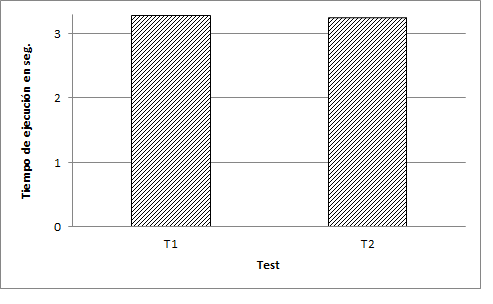
\includegraphics[width=6cm]{./imgs/t1-t2-tiempo}
\caption{Tiempo de ejecución medio con referencia $T_1$.}
\end{figure}
}


\frame{
  \frametitle{Rendimiento de Consultas en SPARQL-Resultados Gráficos}

\begin{figure}[!htb]
\centering
	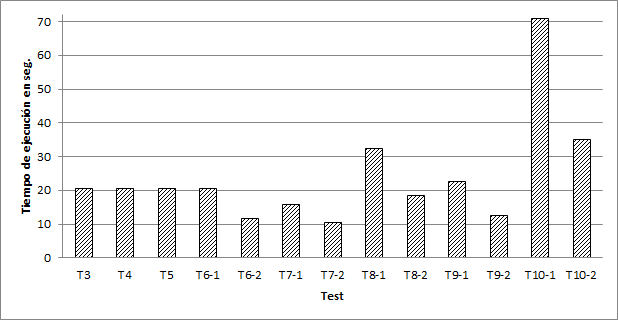
\includegraphics[width=8cm]{./imgs/t3-t10-tiempo}
\caption{Tiempo de ejecución medio con referencia $T_3$.}
\end{figure}
}



\frame{
  \frametitle{Rendimiento de Consultas en SPARQL-Resultados Gráficos}

\begin{figure}[!htb]
\centering
	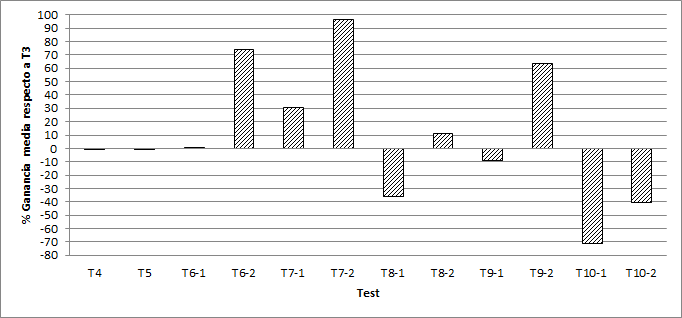
\includegraphics[width=8cm]{./imgs/t3-t10-ganancia}
\caption{Ganancia media con referencia $T_3$ en (\%).}
\end{figure}
}




\frame{
  \frametitle{Rendimiento de Consultas en SPARQL-Resultados}

\begin{block}{Valoración}
 \begin{enumerate}
\item Existen diversas mejoras aplicables a las consultas en SPARQL (LIMIT, FILTER, etc.) que mejoran el rendimiento.
\item El tratamiento $T^{2}_7$ genera el mejor tiempo de ejecución utilizando consultas simples paralelas, con uso de claúsulas LIMIT y FILTER en SPARQL. 
\item La generación de consultas a partir de una expandida no genera sobrecarga significativa en el tiempo de ejecución.
\item Una caché de consultas con resultados predefinidos o índices en el repositorio puede mejorar el rendimiento.
\item Los resultados han implicado una refactorización del código inicial de \texttt{moldeas-api}.
 \end{enumerate}
\end{block}
}
% 
% 
\frame{
  \frametitle{Rendimiento de Consultas en SPARQL-Conclusiones}

\begin{exampleblock}{Puntos Clave}
\begin{itemize}
 \item La \textbf{ejecución} de consultas sobre \textbf{grandes conjuntos de datos} puede ser \textbf{lenta}.
 \item La \textbf{ejecución} de consultas en \textbf{paralelo} \textbf{mejora} el \textbf{tiempo} de ejecución.
 \item El tiempo de generación de las consultas es despreciable.
 \end{itemize}
\end{exampleblock}
}


